%!TEX TS-program = lualatex
\documentclass[a4paper]{friggeri-cv}
\usepackage{afterpage}
\usepackage{hyperref}
\usepackage{color}
\usepackage{xcolor}
\usepackage{smartdiagram}
\usepackage{fontspec}
% if you want to add fontawesome package
% you need to compile the tex file with LuaLaTeX
% References:
%   http://texdoc.net/texmf-dist/doc/latex/fontawesome/fontawesome.pdf
%   https://www.ctan.org/tex-archive/fonts/fontawesome?lang=en
%\usepackage{fontawesome}
\usepackage{metalogo}
% \usepackage{dtklogos}
\usepackage[utf8]{inputenc}
\usepackage{tikz}
\usetikzlibrary{mindmap,shadows}
\hypersetup{
    unicode=true,
    pdftitle={Lei’s Resume},
    pdfauthor={Lei Zhao},
    pdfsubject={},
    pdfkeywords={resume},
    pdfcreator={LuaLaTeX},
    colorlinks=false,           % no lik border color
    allbordercolors=white       % white border color for all
}
\smartdiagramset{
    bubble center node font = \footnotesize,
    bubble node font = \footnotesize,
    % specifies the minimum size of the bubble center node
    bubble center node size = 0.5cm,
    %  specifies the minimum size of the bubbles
    bubble node size = 0.5cm,
    % specifies which is the distance among the bubble center node and the other bubbles
    distance center/other bubbles = 0.3cm,
    % sets the distance from the text to the border of the bubble center node
    distance text center bubble = 0.5cm,
    % set center bubble color
    bubble center node color = pblue,
    % define the list of colors usable in the diagram
    set color list = {lightgray, materialcyan, orange, green, materialorange, materialteal, materialamber, materialindigo, materialgreen, materiallime},
    % sets the opacity at which the bubbles are shown
    bubble fill opacity = 0.6,
    % sets the opacity at which the bubble text is shown
    bubble text opacity = 0.5,
}

\addbibresource{bibliography.bib}
\RequirePackage{xcolor}
\definecolor{pblue}{HTML}{0395DE}

\begin{document}
\header{Lei}{Zhao}
      {Polyglot Programmer}
      
% Fake text to add separator      
\fcolorbox{white}{gray}{\parbox{\dimexpr\textwidth-2\fboxsep-2\fboxrule}{%
.....
}}

% In the aside, each new line forces a line break
\begin{aside}
  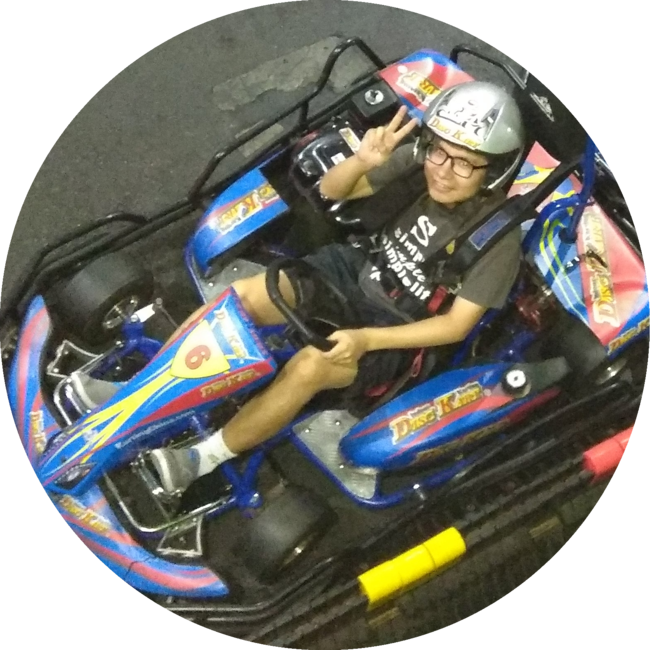
\includegraphics[scale=0.18]{img/zhao_circle.png}
  \section{Address}
  Pudong New Area
  Shanghai, China
  ~
  \section{Tel \& WeChat}
  +1 319 555 0128
  lei.zhao
  ~
  \section{Email}
  \href{mailto:lei.zhao@example.com}{\textbf{lei.zhao@}example.com}
  ~
  \section{SO \& Git}
  \href{https://stackoverflow.com/users/2117531/lei-zhao}{stackoverflow.com/u/2117531}
  \href{https://github.com/LeeiFrankJaw}{github.com/LeeiFrankJaw}
  ~
  % use  \hspace{} or \vspace{} to change bubble size, if needed
  \section{Programming}
  \smartdiagram[bubble diagram]{\textbf{Python},\textbf{\scriptsize JavaScript},\textbf{\scriptsize Postgres},\textbf{\hspace{0.8ex}Java\hspace{0.8ex}},\textbf{\hspace{1.1ex}C\hspace{1.1ex}},\textbf{\tiny \hspace{0.4ex}Clojure\hspace{0.4ex}}}
  ~
  % \section{Personal Skills}
  % \smartdiagram[bubble diagram]{\textbf{Problem}\\\textbf{Solving},\textbf{\hspace{0.5ex}Curiosity\hspace{0.5ex}},\textbf{Organize},\textbf{\scriptsize\hspace{0.2ex}Manage\hspace{0.2ex}},\textbf{\scriptsize Initiative},\textbf{\tiny Team}\\\textbf{\tiny Player}}
  % ~
  \section{OS Preference}
  \textbf{GNU/Linux}
\includegraphics[scale=0.40]{img/5stars.png}
  \textbf{BSD}
\includegraphics[scale=0.40]{img/4stars.png}
  \textbf{Windows}
\includegraphics[scale=0.40]{img/3stars.png}
  \textbf{macOS}
\includegraphics[scale=0.40]{img/2stars.png}
  ~
  \section{Languages}
  \textbf{Chinese}
\includegraphics[scale=0.40]{img/5stars.png}
  \textbf{English}
\includegraphics[scale=0.40]{img/4stars.png}
  \textbf{Russian}
\includegraphics[scale=0.40]{img/1stars.png}
  ~
\end{aside}
~
\section{Experience}
\begin{entrylist}
  \entry
  {02/17 - 12/17}
  {Python programmer}
  {\href{https://www.mesoor.com/}{Mesoor}}
  {I wrote web crawler using pyspider to crawl job descriptions from several major Chinese employment-related website like \href{https://www.lagou.com/}{lagou.com}, \href{https://www.zhaopin.com/}{zhaopin.com}, \href{http://www.chinahr.com/}{chinahr.com}, and so on so forth.  I implemented an automatic login service using w3c \href{https://github.com/w3c/web-platform-tests/pull/6743}{web driver} technology and help our client import their resumes into our own system.  I also participated in a lot front-end website development with both angular/typescript and vanilla javascript and some back-end development with flask and hug.  I was also often assigned tasks related to database (PostgreSQL primarily, also MySQL) operation and migration.  \\}
  \entry
  {11/14 - 02/15}
  {Clojure programmer}
  {\href{http://www.starworking.com/}{Starworking}}
  {Develop full-stack website with Clojure and related technology while learning Clojure on the go.}
\end{entrylist}
\\
\section{Education}
\begin{entrylist}
  \entry
  {09/14 - 06/17}
  {Zhuanke Certificate of Graduation in Computer Science}
  {SJTU}
  {This certificate, which I attained by self-taught examination, is equivalent to an Associate's degree.  Upon completion, I learned C, RDBMS, data structures, discrete math, computer organization, operating system, networking, digital logic, 8086 interfacing, and so on.\\}
  \entry
  {08/11 - 02/12}
  {Computer Science}
  {Cornell College}
  {Since I had only one semester here, I learned about Java and formal logic, and became an Emacs and Linux user.}
\end{entrylist}

% \begin{aside}
%   ~
%   ~
%   ~
%   % \section{Places Lived}
%   %   \includegraphics[scale=0.25]{img/italia.png}
%   %   ~
% \end{aside}

% \section{Publications}
% Author, Author, Author\\
% \textbf{Lorem ipsum dolor sit amet, consectetur adipiscing elit, sed do eiusmod tempor incididunt ut labore et dolore magna aliqua}\\
% \emph{Lorem ipsum dolor sit amet, consectetur adipiscing elit, sed do eiusmod tempor incididunt ut labore et dolore magna aliqua}
% \\
\section{Honors \& Awards}
\begin{entrylist}
  \entry
    {11/09}
    {2nd Prize in NOIP}
    {China Computer Federation}
    {NOIP is an annual competitive programming competition for secondary school students.  The contest consists of five hours of computer programming on an individual basis, solving problems of an algorithmic nature.}
\end{entrylist}

% \newpage

\section{Certifications}
\begin{entrylist}
  \entry
  {05/15}
  {\href{https://s3.amazonaws.com/verify.edx.org/downloads/5eb2696ec8874930bb0fda0b8b6756b6/Certificate.pdf}{Linear Algebra - Foundations to Frontiers}}
  {edX}
  {This was my first exposure to MATLAB and I learned about FLAME methodology for systematically developing dense linear algebra library.\\}
  \entry
  {04/15}
  {\href{https://s3.amazonaws.com/accredible_user_certificate/certificates/144339/original/Coursera_matrix_2015.pdf}{Coding the Matrix: Linear Algebra through Computer Science Applications}}
  {Coursera}
  {I learned many applications of linear algebra in a variety of fields like computer vision, cryptography, graphics, information retrieval, and so on.\\}
\end{entrylist}
\begin{entrylist}
  \entry
  {09/14}
  {\href{https://s3.amazonaws.com/accredible_user_certificate/certificates/53611/original/Coursera_hwswinterface_2014.pdf}{The Hardware/Software Interface}}
  {Coursera}
  {I learned key computational abstraction levels below modern high-level languages, number representation, assembly language, memory management, the operating-system process model, high-level machine architecture including the memory hierarchy, and how high-level languages are implemented.  I was very sad to know in 2015 that Prof. Borriello passed away after six-year fight against colon cancer.}  
  \entry
  {06/14}
  {\href{https://www.coursera.org/account/accomplishments/records/jeAXpfyLDdj7TBYK}{Functional Programming Principles in Scala}}
  {Coursera}
  {In addition to some hands-on experiences with Scala, I learned about proofs of invariants for functional programs and how to trace execution symbolically.\\}
  \entry
  {06/14}
  {\href{https://www.coursera.org/account/accomplishments/records/AqU3pfW4qRTd8FzE}{Logic: Language and Information 2}}
  {Coursera}
  {This is my first officially verified MOOC.  I learned various application of formal logic in different fields such as EE, CS, linguistics, philosophy, and math.  Specifically, I learned Robinson's unification and resolution and played with SWI-Prolog.  This course also deepened my understanding of \(\epsilon\textit{-}\delta\) language often seen in mathematical analysis.\\}
  \entry
  {06/13}
  {\href{https://s3.amazonaws.com/verify.edx.org/downloads/eedec1d10b884139876bee106313142c/Certificate.pdf}{Introduction to Computer Science and Programming}}
  {edX}
  {This course broadened my horizons and introduced me to many topics in computer science.\\}
  \entry
  {11/12}
  {\href{https://s3.amazonaws.com/accredible_user_certificate/certificates/48300/original/IntroLogic.pdf}{Introduction to Logic}}
  {Coursera}
  {I was one of earliest MOOC learners in China.  Perhaps due to my life-long interest in formal logic, this course was one of my first MOOCs.}
\end{entrylist}

% \section{Other Info}
% For the Italian job market:\\
% \emph{Si autorizza il trattamento delle informazioni contenute nel curriculum in conformità alle disposizioni previste dal d.lgs. 196/2003. Si dichiara altresì di essere consapevole che, in caso di dichiarazioni non veritiere, si è passibili di sanzioni penali ai sensi del DPR 445/00 oltre alla revoca dei benefici eventualmente percepiti.}
% \\
% \begin{flushleft}
% \emph{Dec 12th, 2017}
% \end{flushleft}
% \begin{flushright}
% \emph{Lei Zhao}
% \end{flushright}

\end{document}

% Local Variables:
% TeX-engine: luatex
% End:
